\documentclass{standalone}
\usepackage{tikz}
\usetikzlibrary{positioning, arrows.meta}

\begin{document}
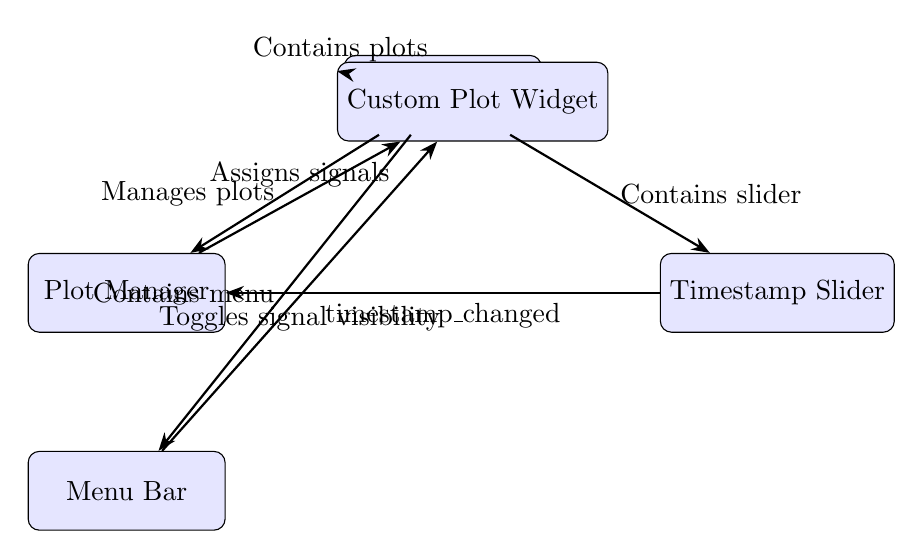
\begin{tikzpicture}[
    node distance=2cm,
    box/.style={draw, fill=blue!10, rounded corners, minimum width=2.5cm, minimum height=1cm},
    arrow/.style={->, thick, >=Stealth},
]

% Nodes
\node[box] (mainwindow) {Main Window};
\node[box, below left=1.5cm and 1.5cm of mainwindow] (plotmanager) {Plot Manager};
\node[box, above right=of plotmanager] (customplot) {Custom Plot Widget};
\node[box, below right=1.5cm and 1.5cm of mainwindow] (slider) {Timestamp Slider};
\node[box, below=1.5cm of plotmanager] (menubar) {Menu Bar};

% Arrows between nodes
\draw[arrow] (mainwindow) -- (plotmanager) node[midway, left] {Manages plots};
\draw[arrow] (mainwindow) -- (customplot) node[midway, above] {Contains plots};
\draw[arrow] (mainwindow) -- (slider) node[midway, right] {Contains slider};
\draw[arrow] (mainwindow) -- (menubar) node[midway, left] {Contains menu};

\draw[arrow] (slider) -- (plotmanager) node[midway, below] {timestamp\_changed};
\draw[arrow] (plotmanager) -- (customplot) node[midway, above] {Assigns signals};
\draw[arrow] (menubar) -- (customplot) node[midway, below] {Toggles signal visibility};

\end{tikzpicture}
\end{document}
